\section{Introduzione ai multiprocessori}\label{capitolo8}
Negli ultimi quindici anni siamo entrati in una nuova era delle architetture dei calcolatori, i multiprocessori ora sono i più diffusi sia in ambito embedded che in quello general-purpose, in quanto forniscono elevate prestazioni, scalabilità ed affidabilità. Si parla di multiprocessori quando si hanno dei computer con più processori strettamente accoppiati i quali sono coordinati e controllati dal sistema operativo e condividono la memoria e lo spazio degli indirizzi. Si parla, invece, di multicores quando più core risiedono sullo stesso chip.\\
I multiprocessori comportano una serie di problematiche che spaziano dal metodo di collegamento a problemi di coordinamento; il primo problema che ci poniamo è come connettere i diversi processori. Esistono due soluzioni principali, la prima prevede l'utilizzo di un singolo bus come quello mostrato in \figurename\,\ref{fig:multisinglebus} dove il mezzo di connessione (il \emph{bus}) è situato tra i processori e la memoria ed esso viene utilizzato ogni qualvolta sia necessario un accesso in memoria; questo meccanismo tuttavia comporta alcune problematiche prima tra tutte l'impossibilità di connettere una serie infinita di processori ma solamente un numero limitato causando problemi di \emph{saturazione}.
\begin{figure}[htb]
\centering
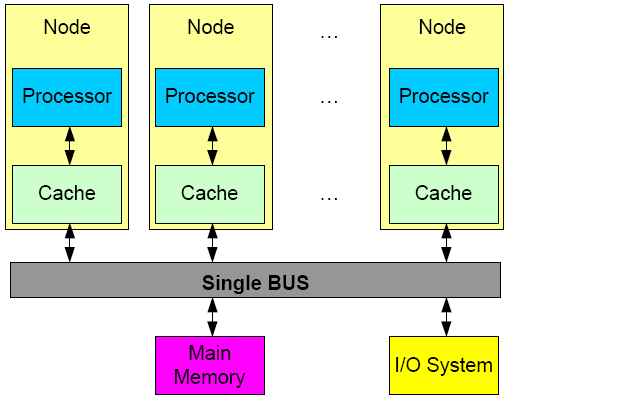
\includegraphics[scale=0.5]{img/multisinglebus.png}
\caption{Architettura multiprocessore a singolo bus}\label{fig:multisinglebus}
\end{figure}
Una seconda tipologia, mostrata in \figurename\,\ref{fig:multinetwork} di collegamento tra diversi processori è quella che utilizza una \emph{rete} nella quale ogni processore ha a disposizione una sua parte di memoria e la rete connette solamente i nodi i quali si scambiano comunicazione interprocesso. 
\begin{figure}[htb]
\centering
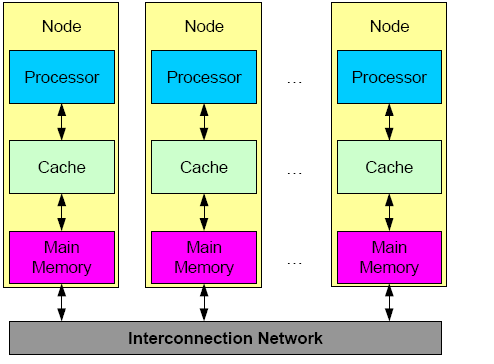
\includegraphics[scale=0.5]{img/multinetwork.png}
\caption{Architettura multiprocessore con connessione tramite rete}\label{fig:multinetwork}
\end{figure}
Per quanto riguarda la tipologia di connessione esistono diverse topologie che la rete può assumere, la forma e le interconnessioni dipendono da un treade-off tra costi e prestazioni, una rete completamente connessa è molto performante tuttavia è anche molto costosa. Alcuni esempi di topologia di reti sono:
\begin{description}
\item[Single bus]
\item[Anello]
\item[Maglia]
\item[N-cubo]
\item[Completamente connessa]
\end{description}
Per descrivere una rete si possono utilizzare dei grafici come quello di \figurename\,\ref{fig:networking} che rappresenta una rete ad anello nei quali i \emph{nodi}, rappresentati dai quadrati sono i nodi che comprendono processore e memoria, i cerchi rappresentano invece gli \emph{switch} che connettono i nodi alla rete. Gli \emph{archi} invece rappresentano le linee di comunicazione tra gli switch e sono sempre di tipo bidirezionale. Il costo di una rete è definito dal numero di \emph{switch}, dal numero di archi che connettono i diversi switch, dalla lunghezza dei collegamenti.\\
\begin{figure}[htb]
\centering
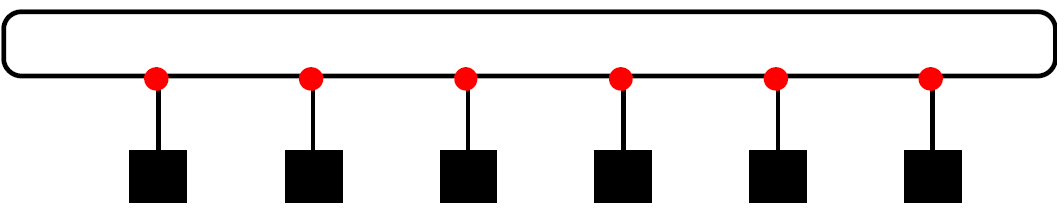
\includegraphics[scale=0.5]{img/networking.png}
\caption{Esempio di rete ad anello}\label{fig:networking}
\end{figure}
Per analizzare le performance di una determinata tipologia di rete introduciamo due metriche di riferimento, una che analizza il caso migliore ed una che analizza il caso peggiore. Il caso migliore è dato dal \emph{total network bandwidth} ovvero la capacità massima di trasferimento che è data dalla banda di ogni link moltiplicata per il numero di link. Definendo:
$$P = \# \ di \ nodi$$
$$b = banda \ del \ singolo \ link$$
Per una rete a singolo bus abbiamo che nel caso migliore la banda della rete è data dalla massima banda del link $(1 \times b)$; per una rete ad anello invece la massima banda è data dal numero di nodi moltiplicato per la banda di un link $(P \times b)$.
Nel caso peggiore invece si considera la rete divisa in due parti ognuna delle quali con la metà dei nodi e si sommano le capacità dei link che attraversano l'immaginaria linea di separazione dei nodi; si ha così che per la rete ad anello la banda diventa $(2 \times b)$ mentre per la rete a singolo bus rimane invariata $(1 \times b)$. Nel caso di reti non simmetriche dobbiamo considerare la divisione che da le peggiori performance per la rete.\\
Analizziamo ora una rete di tipo \emph{completamente connessa} nel quale ogni nodo è connesso ad ogni altro nodo da un link bidirezionale; tale struttura ha un costo molto alto ma le sue performance sono ottime. La banda totale è data da $\{(P \times (P-1))/2\}\times b$ mentre il caso peggiore è dato da $(P/2)^2 \times b$.\\
Nel caso di topologia a maglia come quella di \figurename\,\ref{fig:mesh} abbiamo che dati $P$ nodi possiamo individuare un numero $N = \sqrt{P}$ che è la dimensione della maglia il numero di canali di comunicazione è dato da $N \times (N-1)$ canali orizzontali e $N \times (N-1)$ canali verticali per ogni switch interno abbiamo che il numero di link è pari a \emph{5} (4 provenienti dagli altri switch e uno proveniente dal nodo) mentre per gli switch sul bordo abbiamo che il numero di link è pari a \emph{3}. La banda nel caso migliore è data da $\{2 * N * (N-1)\}\times b$ mentre nel caso peggiore è data da $N \times B$.\\
\begin{figure}[htb]
\centering
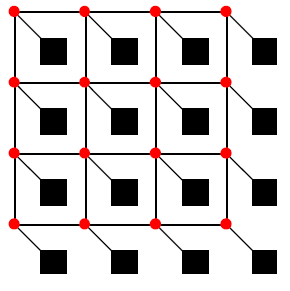
\includegraphics[scale=0.5]{img/mesh.png}
\caption{Esempio di topologia a maglia con N=4}\label{fig:mesh}
\end{figure}
Nel caso in cui la topologia sia di tipo iper-cubica il numero di nodi determina la dimensione del cubo tramite la formula $P = 2^N$ in \figurename\,\ref{fig:hypercube} vediamo la configurazione di un ipercubo con $P=16$ ogni nodo a un numero di vicini pari ad \emph{N} e ogni switch ha esattamente $N+1$ link. La banda totale di questa configurazione è data dalla formula $\{(N \times P)/2\}\times b$ mentre la bada di bisezione è data da $2^{n-1} \times b$.
\begin{figure}[htb]
\centering
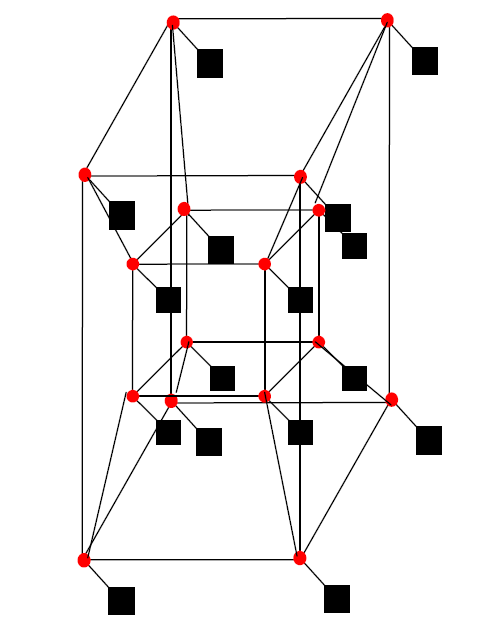
\includegraphics[scale=0.5]{img/hypercube.png}
\caption{Esempio di topologia ad ipercubo.}\label{fig:hypercube}
\end{figure}
\subsection{Gestione della memoria}
In questo paragrafo ci chiediamo come i diversi processi possono condividere i dati e come possono gestire la memoria.
Partiamo con l'analizzare come i diversi processori condividono lo memoria, tale condivisione può avvenire in due modi tramite il \emph{modello di memoria a spazio degli indirizzi}, il primo modo è avere un singolo spazio degli indirizzi condiviso mentre il secondo è avere più spazi degli indirizzi logicamente separati come mostrato in \figurename\,\ref{fig:adressspace}.
\begin{figure}[htb]
\centering
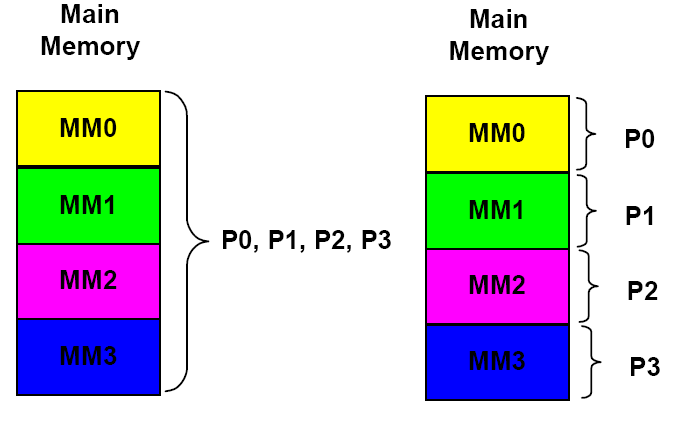
\includegraphics[scale=0.5]{img/addressspace.png}
\caption{Esempio di singolo spazio degli indirizzi condiviso e spazio degli indirizzi multiplo.}\label{fig:adressspace}
\end{figure}
Nel caso di singolo spazio degli indirizzi condiviso un qualsiasi processo può fare riferimento a qualsiasi area di memoria, gli indirizzi sono condivisi tra i processi ed un indirizzo fisico su due processi diversi fa riferimento alla stessa area di memoria. La comunicazione tra processi e thread avviene tramite lo spazio di memoria condiviso, la gestione delle comunicazione è implicita e avviene tramite l'utilizzo delle operazioni di load e di store. Una memoria condivisa non implica necessariamente che esista un unica memoria centrale. Questo tipo di modello tuttavia comporta problemi di coerenza della cache.\\
Nel caso di spazio degli indirizzi multiplo i processi comunicano tra di loro tramite le primitive \texttt{send} e \texttt{recive}; lo spazio di memoria è logicamente diviso e quindi due processi non potranno mai fare riferimento alla stessa area di memoria. La gestione della comunicazione tra i processi è gestita in modo esplicito tramite l'utilizzo delle primitive \emph{send} e \emph{recive}, la memoria di un processo non può essere acceduta da un altro processo se esso non è supportato dal protocollo software evitando così problemi di cache coerence.\\
Un altro problema riguardante la gestione della memoria nei sistemi multiprocessore è quello di dove posizionare fisicamente la memoria. Esistono due possibilità, la prima, mostrata in \figurename\,\ref{fig:memcenter} prevede di posizionare la memoria all'esterno dei nodi in un punto accessibile da tutti i processori. Nel secondo caso, mostrato in \figurename\,\ref{fig:memdist} prevede di suddividere la memoria su ogni singolo nodo.\\
\begin{figure}[htb]
\centering
\subfigure[memcenter]{
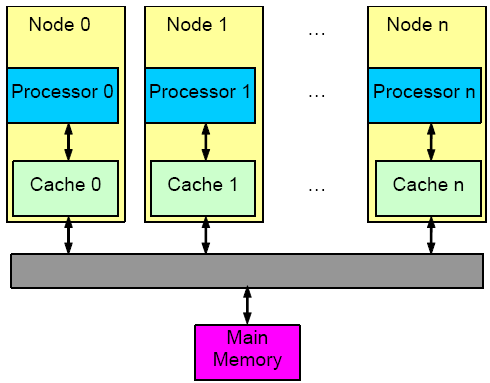
\includegraphics[scale=0.5]{img/memcenter.png}
\label{fig:memcenter}
}
\subfigure[memdist]{
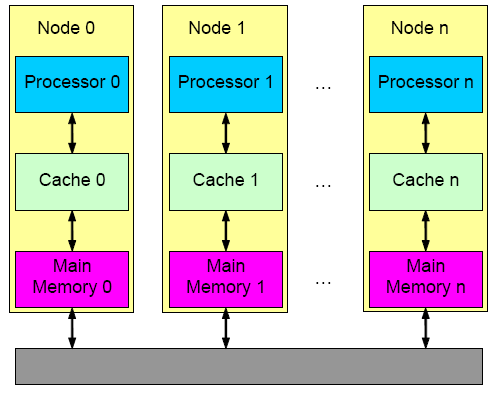
\includegraphics[scale=0.5]{img/memdist.png}
\label{fig:memdist}
}
\end{figure}
Nel caso di memoria centrale si parla di \textbf{UMA} (\emph{Uniform Memory Access}) il tempo di accesso alla memoria è uniforme per tutti i processori indipendentemente da quale sia il processo e da quale area di memoria esso richieda. Nel caso invece di memoria condivisa si parla di \textbf{NUMA} (\emph{Non Uniform Memory Access}) in questo caso il tempo di accesso dipende dalla posizione di memoria che si richiede e da posizione del processore.\\
Nella maggior parte dei sistemi multiprocessore attuali troviamo una struttura con singolo spazio degli indirizzi e una memoria centrale che permette un accesso a memoria uniforme, tali processori sono anche chiamati \emph{Symmetric Multiprocessor (SMPs)}. La maggior parte dei processori \emph{multicore} attualmente esistenti sono di tipo SMPs con un ridotto numero di cores ($\leq 8$) tipicamente esiste un livello di cache condiviso e uno o più livelli di cache privati per ogni core.\\
Quando il numero di core invece aumenta ogni risorsa centralizzata del sistema diventa un collo di bottiglia. Per incrementare la banda di comunicazione si utilizzano bus multipli o reti di comunicazione dove le memorie condivise sono configurate come banchi di memoria multipli. Un esempio di questa architettura è mostrato in \figurename\,\ref{fig:dsmarch} dove ogni processore condivide l'intero spazio di memoria tuttavia il tempo di accesso dipende dalla posizione alla quale si vuole accedere (\emph{NUMA}); l'accesso al banco di memoria connesso direttamente al processore è molto più veloce rispetto agli altri.
\begin{figure}[htb]
\centering
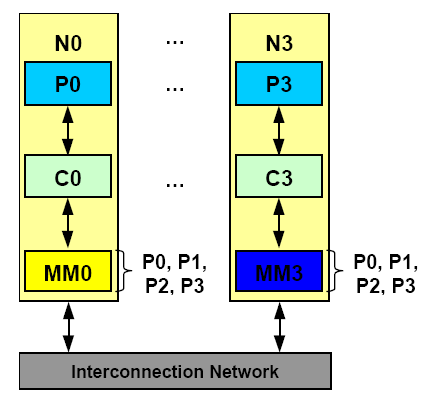
\includegraphics[scale=0.5]{img/dsmarch.png}
\caption{Architettura di un sistema multiprocessore a memoria distribuita}\label{fig:dsmarch}
\end{figure}
Negli ultimi anni si sono affermati una nuova tipologia di computer multiprocessore, i \emph{cluster} composti da computer individuali con spazi di memoria privati e l'interconnessione avviene tramite il passaggio di messaggi.\\
Esistono alcuni limiti al parallelismo tra processi, il primo è quello dovuto alla quantità di parallelismo che si può estrapolare tramite il compilatore. Il secondo limite dipende molto dai costi di comunicazione infatti, un accesso a memoria tra cores sullo stesso chip è dell'ordine dei 35-50 cicli mentre si aggira tra i 100 e i 500 cicli per accessi tra cores su chip differenti. Diventa così molto importante meccanismi di cache, in quanto riducono il tempo medio di accesso, inoltre riducono i problemi di contesa in quanto permettono la copia dei dati, tuttavia questo porta a problemi di \emph{coerenza} della cache.\\
Per sopperire ai problemi di coerenza della cache esistono diversi meccanismi i principali sono:
\begin{description}
\item[Migrazione:] che consiste nello spostamento dei dati che permette un accesso molto rapido.
\item[Replicazione:] consiste nel creare molte copie dei dati riducendo così la contesa su di essi.
\end{description}
Per assicurare la coerenza si utilizzano dei \emph{protocolli di coerenza}, possiamo distinguere due classi di protocolli di coerenza:
\begin{description}
\item[Snooping protocol:] nei quali ogni core tiene traccia dello stato dei dati su ogni blocco, un controllore (\emph{snoop}) sul bus controlla le richieste dirette ad altre cache.
\item[Directory-based protocol:] lo stato di ogni blocco di memoria è mantenuto in un punto denominato \emph{directory} che può essere un unico punto nel caso di SMP o multiplo in caso di DSM.
\end{description}
Analizzeremo i protocolli di coerenza più in dettaglio nel paragrafo seguente.\\
L'ultima problematica che ci poniamo è quella di come sincronizzare e coordinare i diversi processori. Esistono diversi modelli di comunicazione alcuni già visti come la \emph{memoria condivisa} tramite cui i processori comunicano utilizzando uno spazio degli indirizzi condiviso, tale modello è di facile implementazione e adatto un ridotto numero di macchine in quanto facile da implementare con bassa latenza e permette di utilizzare i controlli di coerenza dell'hardware. Il secondo modello è quello del \emph{passaggio di messaggi} in questo caso è adatto a processori con meccanismi di memoria privati richiede un hardware minore e si concentra sull'ottimizzazione dei costi sulle operazioni non locali. L'ultimo modello è il \emph{data parallel} in questo caso si adatta ad operazioni che possono essere eseguite in parallelo su un numero molto grande di strutture dati come gli \emph{array}. In questo caso un controllore distribuisce i dati sugli altri processori, i dati sono distribuiti su tutte le memorie. Il principio del \textbf{SIMD} (\emph{Single Instruction Multiple Data}) ha portato allo sviluppo della programmazione di dati parallela nella quale tutti i processori eseguono uno stesso programma.
\subsection{Il problema della coerenza della cache}
Come abbiamo visto nel paragrafo precedente il fatto di avere della memoria condivisa pur avendo della cache dedicata ad ogni processore può portare ad avere problemi di coerenza in quanto un dato in una cache può essere replicato più volte, in quanto questo meccanismo permette di ridurre le contese dovute a letture su dati condivisi.\\
Un meccanismo per ridurre i problemi di coerenza della cache è quello di forzare l'accesso a memoria centrale per i dati condivisi, questo però riduce notevolmente le prestazioni. I problemi di coerenza si possono verificare solamente quando si svolgono delle \emph{read} o delle \emph{write}, tuttavia, l'accesso in lettura a più copie non crea problemi di coerenza, ma il processore deve avere accesso esclusivo quando accede in scrittura. Un processore deve avere la copia più recente di un dato prima di accedervi in lettura così ogni processore deve avere il nuovo valore quando si effettua una scrittura.\\
Per evitare i problemi di coerenza bisogna effettuare due operazioni, la prima è tenere traccia di tutte le copie cahce di un particolare dato condiviso e la seconda è che una scrittura su di un dato condiviso deve o \emph{invalidare}  oppure \emph{aggiornare} tutte le altre copie condivise. La soluzione sono i \emph{protocolli di coerenza}, esistono due classi di protocolli, gli \emph{snooping protocols} e \emph{directory-based protocol}.
Nel caso di protocolli di \emph{snooping} ogni processore tiene traccia dello stato delle condivisione di ogni blocco di memoria ad esso associato, un controllore sul bus denominato \emph{snoop} verifica eventuali richieste indirizzate ad altre cache. Un esempio di questo meccanismo è rappresentato in \figurename\,\ref{fig:snoopprot}
\begin{figure}[htb]
\centering
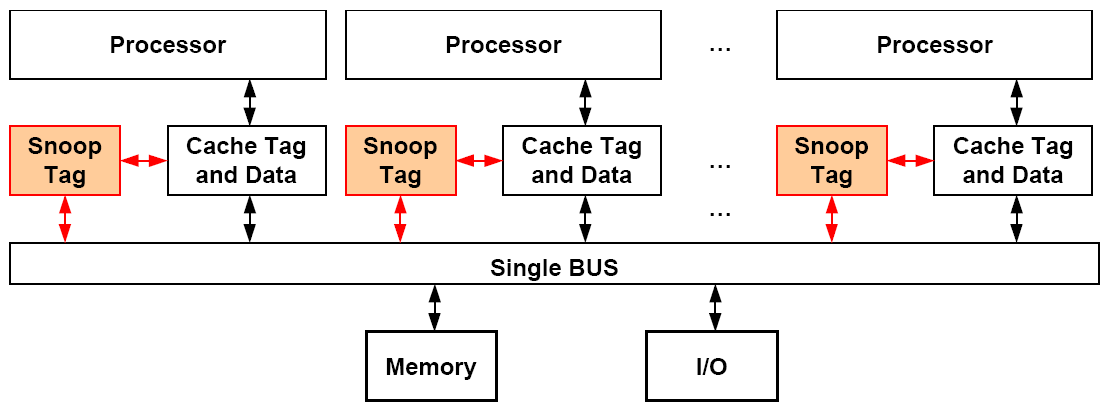
\includegraphics[scale=0.5]{img/snoopprot.png}
\caption{Struttura di uno snooping protocol}\label{fig:snoopprot}
\end{figure}
Ad ogni richiesta sul bus lo \emph{snoop} controlla se è in possesso di una copia del blocco richiesto e risponde di conseguenza, ogni cache che ha una copia del blocco condiviso ha anche una copia del suo stato così facendo non esiste un'entità centrale nel quale lo stato è mantenuto. Le richieste per dei dati condivisi vengono inviati a tutti i processori, le richieste vengono inviate in \emph{broadcast} fino a quando non il processore non riesce a ricostruire le informazioni. Questo tipo di meccanismo è molto adatto per sistemi a memoria centrale condivisa e in particolare per multiprocessori di piccole dimensioni con \textbf{single snoopy bus}. Tuttavia questa tecnica presenta anche alcuni problemi, ogni qualvolta si cerca un blocco condiviso è necessario controllare i \emph{tag} della cache e questo comporta delle interferenze con le normali operazioni del processore in quanto la cache risulta non disponibile. Per evitare questo problema si possono duplicare i tag in modo da poter effettuare le attività di \emph{snooping} per fare ciò è sufficiente aggiungere alla parte dei tag una porta in lettura.\\
Possiamo distinguere due sotto categorie di snooping protocol in base a quello che succede quando si effettua un'operazione di write; le strategie sono due:
\begin{itemize}
\item \textbf{Write-Invalidate Protocol}
\item \textbf{Write-Update Protocol}
\end{itemize}
Nel primo caso  quando un processore scrive in un blocco condiviso esso invia un segnale di \emph{invalidazione} sul bus che fa si che tutte le copie nelle altre cache siano invalidate prima di aggiornare la propria copia locale, il processore è libero di aggiornare il suo dato fino a quando un'altra cache non richiederà il dato. All'arrivo di un segnale di invalidazione ogni cache controlla se ha una copia del dato e in caso affermativo lo marca come non valido. Questo schema permette di avere delle operazioni di lettura simultanee ma solamente una scrittura per volta. Il bus viene utilizzato solamente durante la prima operazione di write effettuata da un processore tutte le altre risultano trasparenti. Questo tipo di protocollo fornisce dei vantaggi paragonabili a quelli del protocollo \emph{write-back} in termini di riduzione di utilizzo del bus.\\
Nel caso di \emph{write-update}, invece, si ha che il processore distribuisce il nuovo valore sul bus e tutte le altre cache verificano la presenza del dato nella loro memoria e in caso affermativo aggiornano con il nuovo valore, in questo modo tutte le copie sono sempre aggiornate ma questo meccanismo richiede un continuo broadcast dei nuovi valori sul bus. Questo protocollo è simile al \emph{write-through} in quanto tutte le scritture effettuano una comunicazione sul bus. Questo protocollo ha il vantaggio di tenere tutte le copie aggiornate e così facendo permette di ridurre la latenza.\\
La maggior parte dei prodotti commerciali attualmente utilizza una cache di tipo \emph{write-back} per ridurre il traffico sul bus e uno snooping protocol di tipo \emph{write-invalidate} l'unico problema che rimane da risolvere è la serializzazione delle scritture in quando il bus è un punto di \emph{arbitrarietà}.\\
Per ogni blocco di memoria possiamo definire tre stati:
\begin{description}
\item[Shared:] quando tutte le copie cache sono aggiornate al valore di memoria
\item[Modified:] quando esiste un unica cache in cui è presente il valore di memoria
\item[] In nessuna cache.
\end{description}
Per i blocchi in cache possiamo distinguere tre stati:
\begin{description}
\item[Shared:] il blocco è aggiornato e può essere letto
\item[Modified:] il blocco è l'unico aggiornato e può essere scritto
\item[Invalid:] il blocco non contiene dei dati validi 
\end{description}
In \figurename\,\ref{fig:snoopfsm} si possono vedere i diversi stati di un blocco cache e le transizioni da uno stato all'altro
\begin{figure}
\centering
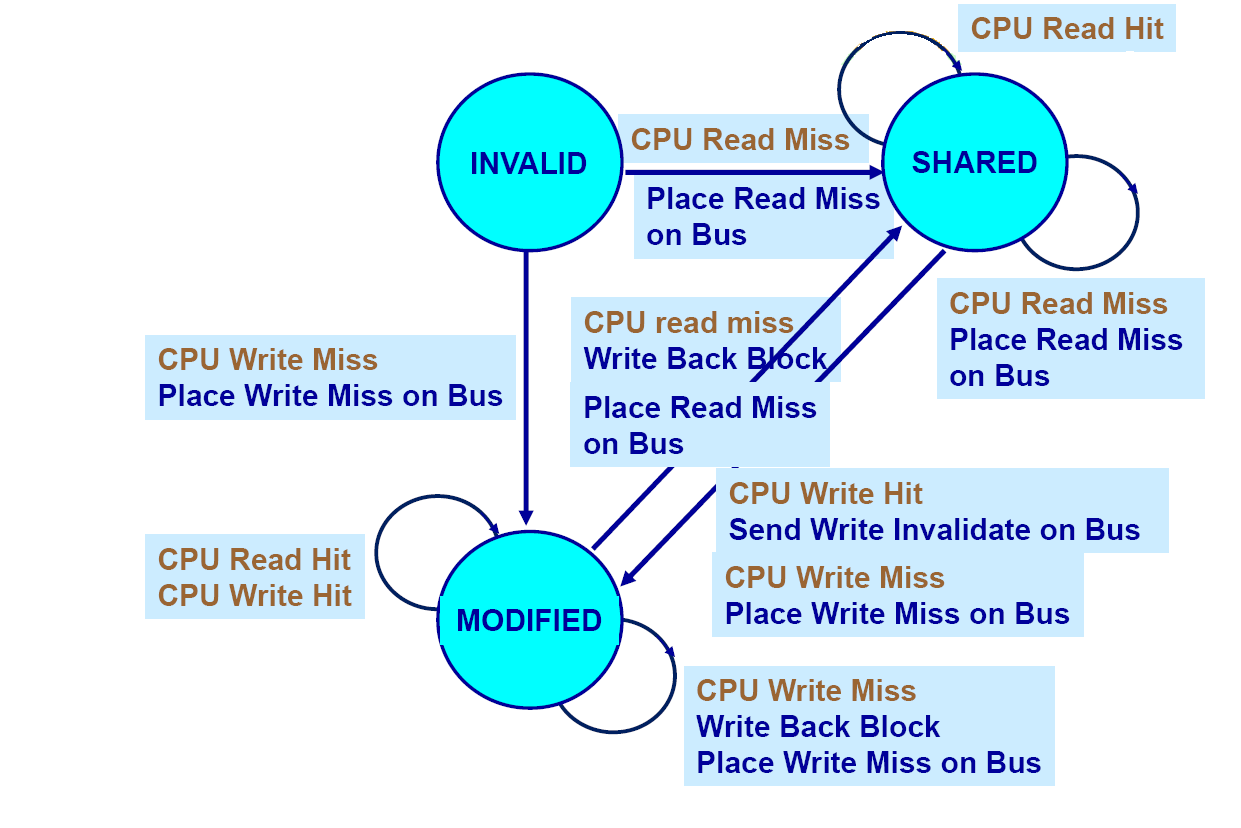
\includegraphics[scale=0.5]{img/snoopfsm.png}
\caption{Macchina a stati finiti che rappresenta un blocco di cache}\label{fig:snoopfsm}
\end{figure}
Un variazione di questo meccanismo prevede per i blocchi di cache un quarto stato, \textbf{Exclusive} in questo caso il blocco non è ancora stato scritto ma è l'unica copia presente nelle cache; tale stato fa si che una successiva scrittura non comporti un invio del segnale di invalidazione sul bus.\\
Analizziamo ora i protocolli \emph{directory based}, lo stato di ogni blocco di memoria fisico è mantenuto in un unico spazio chiamato \emph{directory} ogni riga nella directory corrisponde un blocco di memoria; per quei sistemi con memoria condivisa distribuita anche la directory è distribuita come nel caso di \figurename\,\ref{fig:directorydist} per evitare colli di bottiglia. Questo protocollo risulta più scalare rispetto a quello di snooping. 
\begin{figure}[htb]
\centering
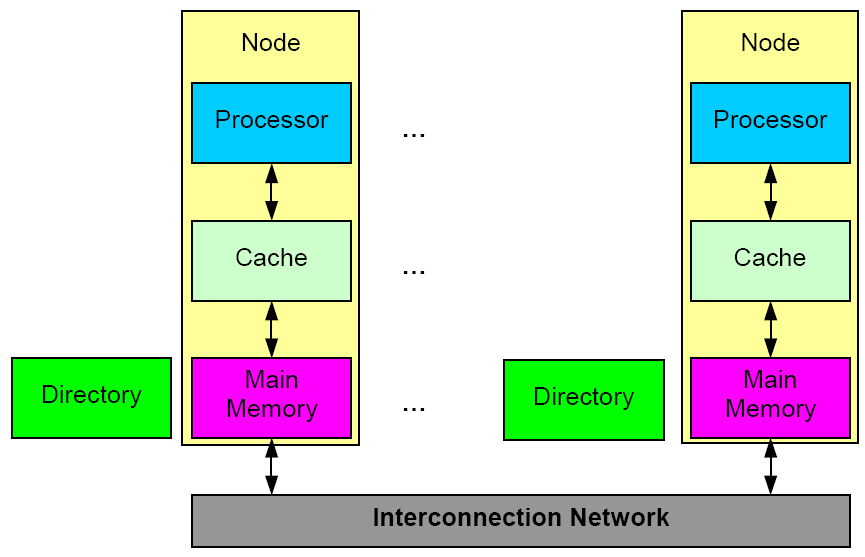
\includegraphics[scale=0.5]{img/directorydist.png}
\caption{Esempio di directory base protocol distribuito}\label{fig:directorydist}
\end{figure}
Le directory mantengono informazioni riguardanti lo \emph{stato} di ogni blocco che può essere:
\begin{description}
\item[Uncached:] ovvero non esistono copie cache valide di quel blocco.
\item[Shared:] uno o più processori mantengono una copia cache aggiornata del dato.
\item[Modified:] solamente un processore (\emph{il possessore}) ha una copia aggiornata del dato, anche la memoria è obsoleta.
\end{description}
Oltre allo stato la directory mantiene un indice del processore o dei processori che hanno una copia del dato imponendo a 1 il campo corrispondente di un vettore di bit come mostrato nell'esempio di \figurename\,\ref{fig:directoryexemp} nel caso in cui il blocco risulti modificato un unico bit del vettore è a 1.
\begin{figure}[htb]
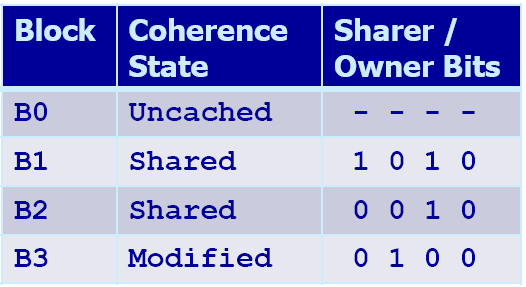
\includegraphics[scale=0.5]{img/directoryexemp.png}
\caption{Esempio di directory per quattro blocchi di memoria utilizzati da quattro processori}\label{fig:directoryexemp}
\end{figure}
Il protocollo directory based sfrutta i \emph{messaggi} per comunicare attraverso i nodi (comunicazione punto-a-punto) ed è necessaria un esplicita risposta dal destinatario questo permette di non avere un unico punto di arbitrarietà.\\
Come per lo snooping protocol anche nel directory based i blocchi in cache possono trovarsi nei tre stati \emph{shared}, \emph{modified} e \emph{invalid}. Solitamente in un protocollo directory based sono coinvolti tre processori:
\begin{description}
\item[Local node:] il nodo da cui la richiesta ha origine.
\item[Home node:] il nodo dove è immagazzinato il dato fisicamente in memoria.
\item[Remote node:] nodo nel quale è presente una copia cache del blocco.
\end{description}
Il \emph{local node} (\textbf{L}) e \emph{home node} (\textbf{H}) possono essere lo stesso nodo, in questo caso la comunicazione può essere di tipo \emph{intra-nodo}. Anche il \emph{remote node} (\textbf{R}) e \textbf{H} possono essere lo stesso nodo. Quello che non può essere è che \textbf{R} ed \textbf{L} siano lo stesso nodo.\\
In \figurename\,\ref{fig:directoryfsm} è mostrato lo stato dei blocchi di memoria con relative richieste provenienti dalle cache nel caso di protocollo directory based.
\begin{figure}[htb]
\centering
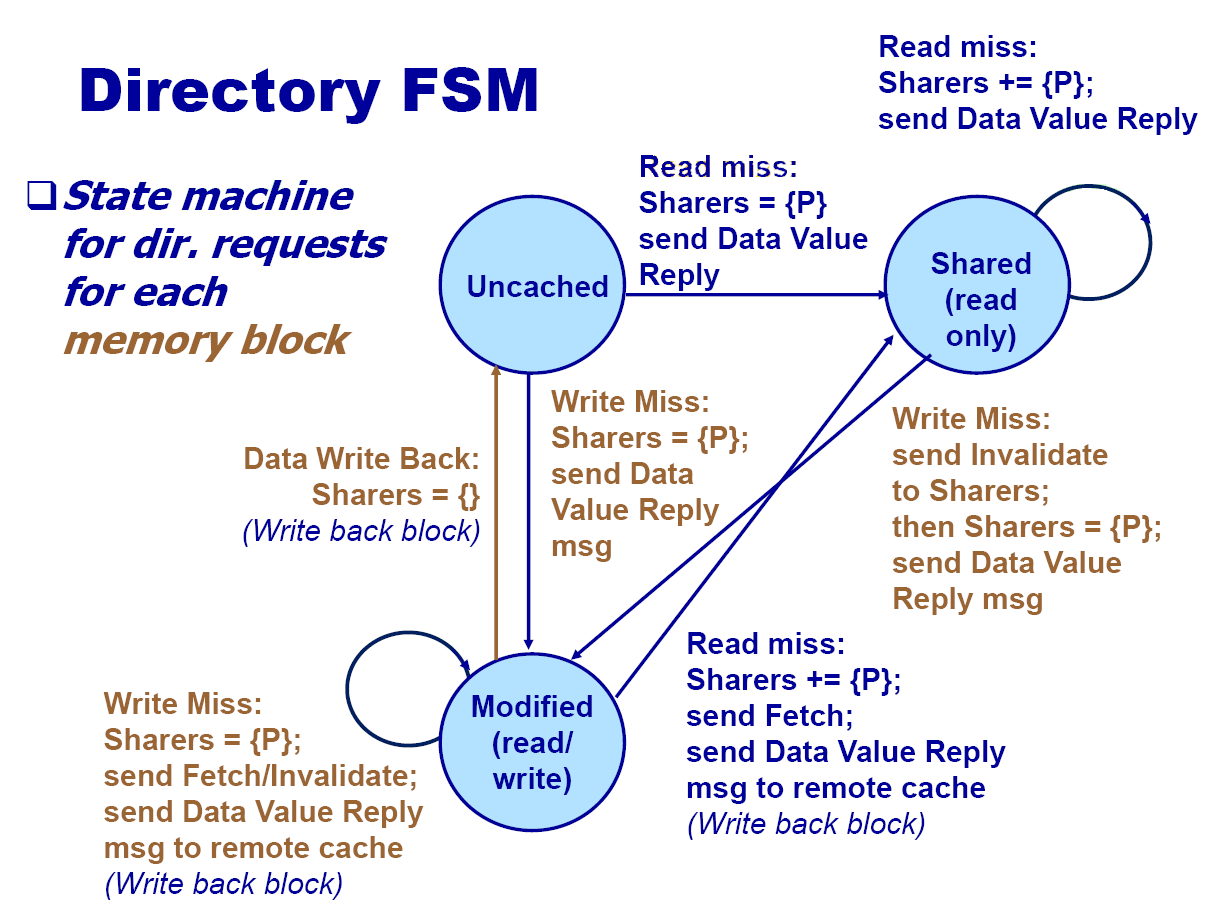
\includegraphics[scale=0.5]{img/directoryfsm.png}
\caption{Macchina a stati finiti per i blocchi di memoria nel caso di protocollo directory based}\label{fig:directoryfsm}
\end{figure}